\documentclass[11pt,a4paper]{article}
\usepackage[margin=2.0cm]{geometry}
\usepackage[T1]{fontenc}
\usepackage{lmodern,amsmath,amssymb,booktabs,array,longtable,graphicx,xcolor,caption,enumitem,microtype,float,tikz,pgfplots}
\usepackage[hidelinks]{hyperref}
\usepgfplotslibrary{groupplots}
\usetikzlibrary{arrows.meta,positioning,shapes.geometric,fit}
\pgfplotsset{compat=1.17}
\captionsetup{font=small,labelfont=bf}
\setlength{\parskip}{4pt}
\definecolor{ok}{RGB}{20,95,50}\definecolor{warn}{RGB}{160,90,0}\definecolor{bad}{RGB}{145,25,25}
\definecolor{cq}{RGB}{200,90,30}\definecolor{cc}{RGB}{40,100,170}\definecolor{cp}{RGB}{150,150,150}
\newcommand{\OK}[1]{\textcolor{ok}{\textbf{#1}}}\newcommand{\WARN}[1]{\textcolor{warn}{\textbf{#1}}}\newcommand{\BAD}[1]{\textcolor{bad}{\textbf{#1}}}
\graphicspath{{gen_v2/}}
\newcommand{\mPimaRBFba}{0.712}
\newcommand{\mPimaStackba}{0.716}
\newcommand{\mPimaAngleba}{0.711}
\newcommand{\mPimaZZba}{0.525}
\newcommand{\mPimaAmpba}{0.530}
\newcommand{\mPimaKothaThrba}{0.741}
\newcommand{\mPimaVQCba}{0.693}
\newcommand{\mPimaHVba}{0.546}
\newcommand{\mPimaFloor}{0.651}
\newcommand{\mSylRFba}{0.925}
\newcommand{\mSylRBFba}{0.923}
\newcommand{\mSylStackba}{0.923}
\newcommand{\mSylAngleba}{0.882}
\newcommand{\mSylZZba}{0.653}
\newcommand{\mSylZZrec}{0.985}
\newcommand{\mSylZZspec}{0.322}
\newcommand{\mSylVQCba}{0.736}
\newcommand{\mSylZZtunedba}{0.848}
\newcommand{\mSylFloor}{0.615}
\newcommand{\mCdcKiranRBFba}{0.727}
\newcommand{\mCdcKiranRBFrec}{0.786}
\newcommand{\mCdcRBFrec}{0.071}
\newcommand{\mCdcRBFba}{0.531}
\newcommand{\mCdcFloor}{0.860}
\newcommand{\mHospBestba}{0.542}
\newcommand{\mHospFloor}{0.912}
\newcommand{\mUpamaSylRFclean}{0.918}
\newcommand{\mUpamaSylRFpaper}{0.981}
\newcommand{\mKothaPimaCleanAcc}{0.763}
\newcommand{\mKothaPimaAUC}{0.825}
\newcommand{\mKiranVQCcleanAcc}{0.694}
\newcommand{\mKiranVQCpaperAcc}{0.675}
\newcommand{\mYoungGMMba}{0.712}
\newcommand{\mYoungGMMrec}{0.876}
\newcommand{\mYoungGMMspec}{0.549}
\newcommand{\mYoungGMMauc}{0.809}
\newcommand{\mYoungGMMacc}{0.663}
\newcommand{\mYadavZpimaAcc}{0.751}
\newcommand{\mYadavZZpimaAcc}{0.658}
\newcommand{\mSodarAmpMinMaxRec}{0.167}
\newcommand{\mSodarAmpStdRec}{0.138}
\newcommand{\mDagaStackGap}{-0.002}
\newcommand{\mDagaStackRec}{0.567}
\newcommand{\mDagaStackAUC}{0.830}
\newcommand{\npimaworse}{9}
\newcommand{\npimabetter}{0}
\newcommand{\npimaNS}{27}
\newcommand{\nsylhetworse}{6}
\newcommand{\nsylhetbetter}{0}
\newcommand{\nsylhetNS}{30}
\newcommand{\ncdcworse}{0}
\newcommand{\ncdcbetter}{11}
\newcommand{\ncdcNS}{25}
\newcommand{\nhospworse}{0}
\newcommand{\nhospbetter}{0}
\newcommand{\nhospNS}{36}
\newcommand{\zhpimaLightGBM}{0.556}
\newcommand{\zhpimaLightGBMGIFweights}{0.585}
\newcommand{\zhsylhetLightGBM}{0.569}
\newcommand{\zhsylhetLightGBMGIFweights}{0.646}

\title{\textbf{Do Quantum Models Help Diagnose Diabetes?}\\[0.2em]\large A plain-language report on eight papers, four diabetes datasets, and what we found (version 2, checked against the executed results)}
\author{Repository: \texttt{Adaptive-Quantum-Kernel-Selection}}
\date{14 November 2026}
\begin{document}\maketitle
\begin{abstract}\noindent
We re-ran the methods of eight published papers on four diabetes datasets (Pima, Sylhet, CDC survey, Hospital 130), each under two test set-ups: the \emph{paper-style} one (copies the paper, including its weak points) and a \emph{clean} one (no information leaks from test to training). \textbf{Main message:} quantum models never beat a plain classical RBF-SVM; two quantum set-ups are clearly worse; very high published accuracies come from leaks or cannot be reproduced; and on imbalanced data most models only guess ``healthy''. All numbers in tables, charts and in the macros come from the result files of the Colab run (\texttt{executed\_results.zip}), not from typing.
\end{abstract}
\tableofcontents\clearpage

\section{The short story}
\begin{enumerate}[leftmargin=1.5em]
\item \textbf{No quantum advantage.} On Pima the plain RBF-SVM gets balanced accuracy \mPimaRBFba; Daga's quantum stacking gets \mPimaStackba and the Angle quantum kernel \mPimaAngleba. These gaps are far smaller than the noise (Holm-corrected $p=1$).
\item \textbf{Some quantum set-ups are clearly worse.} ZZ kernel with default width: \mPimaZZba (Pima) and \mSylZZba (Sylhet); Amplitude kernel and hard voting on Pima are close to coin-flipping too. Tuning the kernel width removes most of the problem (ZZ tuned: \mSylZZtunedba on Sylhet).
\item \textbf{Sylhet looks easy only because of duplicates.} Only 251 of 520 rows are distinct. A random split puts the same patient profile in training and test, so scores jump by 3 to 22 points.
\item \textbf{Uneven groups hide failure.} On CDC, ``always healthy'' already gets \mCdcFloor{} accuracy. The plain RBF-SVM finds only \mCdcRBFrec{} of sick people; most quantum models find none.
\item \textbf{Several headline claims do not reproduce}: Kiran's 99.7\% (we get \mKiranVQCpaperAcc), Kotha's 83.3\% and AUC 1.00 (we get \mKothaPimaCleanAcc{} accuracy, AUC \mKothaPimaAUC), Daga's ZZ and Amplitude accuracies.
\item \textbf{Hospital 130 has almost no signal} for any model: best balanced accuracy is only \mHospBestba{} (0.5 = chance).
\end{enumerate}

\section{What we did}
\begin{figure}[H]\centering
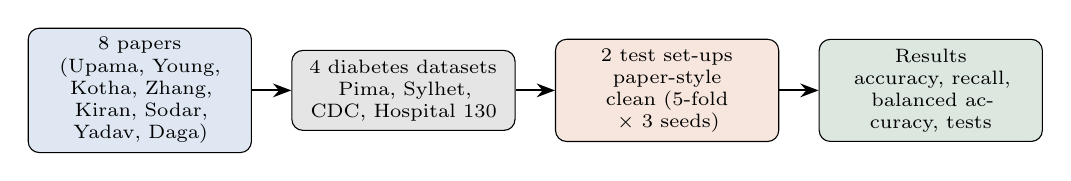
\begin{tikzpicture}[font=\scriptsize,node distance=0.5cm,box/.style={draw,rounded corners,align=center,minimum height=0.9cm,text width=2.6cm,fill=#1},arr/.style={-{Stealth},thick}]
\node[box=cc!15](p){8 papers\\(Upama, Young, Kotha, Zhang,\\Kiran, Sodar, Yadav, Daga)};
\node[box=cp!25,right=of p](d){4 diabetes datasets\\Pima, Sylhet,\\CDC, Hospital 130};
\node[box=cq!15,right=of d](r){2 test set-ups\\paper-style\\clean (5-fold $\times$ 3 seeds)};
\node[box=ok!15,right=of r](o){Results\\accuracy, recall,\\balanced accuracy, tests};
\draw[arr](p)--(d);\draw[arr](d)--(r);\draw[arr](r)--(o);
\end{tikzpicture}\caption{The study design. Quantum models are exact numpy simulations (up to 8 qubits), not real hardware.}\end{figure}
\begin{table}[H]\centering\small\caption{The four datasets (positive class = the group we want to detect).}
\begin{tabular}{lrll}\toprule Dataset & Rows & Positive class & Note\\\midrule
Pima & 768 & diabetes & 34.9\% positive\\
Sylhet & 520 & early-stage diabetes & 61.5\% positive; only 251 distinct rows\\
CDC & 2,000 & self-reported diabetes/prediabetes & random subsample, 14\% positive\\
Hospital 130 & 2,000 & readmitted within 30 days & first visit per patient, 8.8\% positive\\\bottomrule\end{tabular}\end{table}
\textbf{Plain-language glossary.}
\begin{itemize}[leftmargin=1.5em,nosep]
\item \emph{Accuracy}: share of correct answers. Misleading when one group is huge.
\item \emph{Recall}: share of sick people found. \emph{Specificity}: share of healthy people correctly cleared.
\item \emph{Balanced accuracy} = average of recall and specificity. 0.5 means chance. Our main score.
\item \emph{Floor}: accuracy of always guessing the biggest group.
\item \emph{Clean test}: scaling, feature choice and tuning are done only on training data; identical rows never sit on both sides.
\item \emph{Holm-corrected paired test}: a cautious statistical test against RBF-SVM over 15 folds; ``no clear difference'' means we cannot tell the models apart.
\end{itemize}

\section{Results}
\subsection{Every method on every dataset}
\begin{table}[H]\centering\scriptsize\caption{The eight papers: what each method does and what we ran. Quantum models are simulated on a normal computer.}
\begin{tabular}{p{1.3cm}p{5.2cm}p{5.0cm}p{3.6cm}}\toprule Paper & Method we copied & Original data & Quantum? \\\midrule
Upama & Pick the top features with a causal method (DML), then linear SVM, random forest or Angle QSVM & Pima, Sylhet & Angle QSVM only\\
Young & Ensemble of forest, extra-trees and neural net; adds computer-made sick patients (GMM) & Pima & Quantum-inspired, no real circuit\\
Kotha & Random forest; single split vs many splits vs cross-validation & Pima & No\\
Zhang & LightGBM with GIF sample weights when labels are wrong (0--40\%) & Audio data (not used here) & No\\
Kiran & Small 4-qubit circuit (VQC) vs logistic regression and RBF-SVM on the same 4 inputs & Paper: retinopathy images (not used); earlier audit used Pima & VQC\\
Sodar & Angle vs Amplitude quantum kernel & URL-traffic security data (not used here) & Angle, Amplitude\\
Yadav & Z and ZZ quantum kernels; kernel width chosen by inner cross-validation & Breast cancer (WDBC, not used here) & Z, ZZ\\
Daga & Angle, ZZ, Amplitude kernels, RBF-SVM, stacking and voting & Pima & Angle, ZZ, Amplitude\\\bottomrule\end{tabular}\end{table}
\begin{table}[H]\centering\scriptsize\caption{Clean test, mean over 5 folds $\times$ 3 seeds. Each cell is balanced accuracy / recall (0.50 / 0.00 = finds no sick people). Last row: accuracy you get by always guessing the biggest group.}
\begin{tabular}{llcccc}
\toprule & & Pima & Sylhet & CDC & Hosp.\ 130\\
Paper & Method & \multicolumn{4}{c}{balanced acc.\ / recall}\\\midrule
Upama & Angle QSVM, DML top features & 0.72 / 0.56 & 0.90 / 0.93 & 0.50 / 0.00 & 0.50 / 0.00\\
Upama & Random forest, DML top features & 0.73 / 0.60 & 0.91 / 0.95 & 0.58 / 0.21 & 0.50 / 0.01\\
\midrule
Young & QISICGM ensemble + GMM (train folds only) & 0.71 / 0.88 & 0.92 / 0.95 & 0.61 / 0.28 & 0.50 / 0.01\\
\midrule
Kotha & Random forest & 0.73 / 0.60 & 0.92 / 0.94 & 0.56 / 0.14 & 0.50 / 0.00\\
Kotha & Random forest, tuned threshold & 0.74 / 0.76 & 0.91 / 0.91 & 0.72 / 0.75 & 0.54 / 0.44\\
\midrule
Zhang & LightGBM & 0.71 / 0.59 & 0.89 / 0.91 & 0.59 / 0.21 & 0.50 / 0.00\\
Zhang & LightGBM + GIF weights & 0.72 / 0.59 & 0.87 / 0.86 & 0.60 / 0.24 & 0.50 / 0.01\\
\midrule
Kiran & VQC (4 qubits) & 0.69 / 0.69 & 0.74 / 0.76 & 0.72 / 0.71 & 0.54 / 0.50\\
Kiran & RBF-SVM, same 4 PCs, balanced & 0.71 / 0.74 & 0.90 / 0.91 & 0.73 / 0.79 & 0.53 / 0.45\\
\midrule
Sodar & Angle QSVM & 0.71 / 0.55 & 0.88 / 0.92 & 0.50 / 0.00 & 0.50 / 0.00\\
Sodar & Amplitude QSVM (standardised) & 0.53 / 0.14 & 0.80 / 0.90 & 0.50 / 0.00 & 0.50 / 0.00\\
\midrule
Yadav & Z QSVM, width by inner CV & 0.71 / 0.54 & 0.89 / 0.89 & 0.51 / 0.03 & 0.50 / 0.00\\
Yadav & ZZ QSVM (linear), width by inner CV & 0.72 / 0.56 & 0.85 / 0.88 & 0.52 / 0.05 & 0.50 / 0.00\\
\midrule
Daga & Angle QSVM & 0.71 / 0.55 & 0.88 / 0.92 & 0.50 / 0.00 & 0.50 / 0.00\\
Daga & ZZ QSVM (default width) & 0.53 / 0.08 & 0.65 / 0.99 & 0.51 / 0.01 & 0.50 / 0.00\\
Daga & Stacking (OOF, LR meta) & 0.72 / 0.57 & 0.92 / 0.93 & 0.56 / 0.13 & 0.50 / 0.00\\
\midrule
Ref. & RBF-SVM (reference) & 0.71 / 0.56 & 0.92 / 0.94 & 0.53 / 0.07 & 0.50 / 0.00\\
Ref. & Always guess biggest group & 0.50 / 0.00 & 0.50 / 1.00 & 0.50 / 0.00 & 0.50 / 0.00\\
\midrule
\multicolumn{2}{l}{Accuracy of always guessing the biggest group} & 0.65 & 0.62 & 0.86 & 0.91\\
\bottomrule\end{tabular}
\end{table}
\textbf{What the table says, paper by paper.}
\begin{itemize}[leftmargin=1.5em]
\item \textbf{Upama:} the quantum (Angle) and classical versions are about equal on Pima (0.72 vs 0.73) and Sylhet (0.90 vs 0.91). On CDC and Hospital 130 the Angle kernel finds nobody.
\item \textbf{Young:} on real patients the model is fair on Pima (recall 0.88, but many false alarms) and Sylhet (0.92). It is weak on CDC and Hospital 130. Its high paper scores come from made-up rows.
\item \textbf{Kotha:} the plain forest finds few sick people on CDC (0.14). Choosing the decision threshold on training data fixes this (recall 0.75, balanced accuracy 0.72). This is the best CDC result, and it uses no quantum part.
\item \textbf{Zhang:} GIF weights make no clear gain with clean labels (Pima 0.72 vs 0.71; Sylhet slightly worse, 0.87 vs 0.89). Their help is limited to noisy labels, and only on Pima.
\item \textbf{Kiran:} the small quantum circuit is the \emph{worst} of the group on Pima (0.69) and Sylhet (0.74), and ties the classical models on CDC (0.72). The classical RBF-SVM on the same four inputs does as well or better.
\item \textbf{Sodar:} Angle is as good as classical models on Pima and Sylhet. Amplitude is much worse (Pima 0.53, recall 0.14).
\item \textbf{Yadav:} tuning the width makes Z and ZZ about equal to RBF-SVM on Pima. ZZ is a little worse on Sylhet (0.85 vs 0.92).
\item \textbf{Daga:} Angle and stacking match RBF-SVM. ZZ with the default width is bad: Pima 0.53, and on Sylhet it says ``sick'' for almost everyone (recall 0.99, balanced accuracy 0.65).
\item \textbf{By dataset:} Sylhet looks easy (best about 0.92, even with duplicate-aware splits). Pima is middling (best 0.74). CDC works only for methods that handle the rare class on purpose (best 0.73). Hospital 130 is close to chance for all (best 0.54, reached by Kotha's tuned-threshold forest and tied by Kiran's VQC).
\end{itemize}
\textbf{Overall:} no quantum method is clearly better than the classical reference on any dataset. The best result on Pima, Sylhet and CDC comes from a classical model or a classical trick (class weights, threshold choice). On Hospital 130 the best score (0.54) is shared by a classical and a quantum model, and it is barely above chance.

\subsection{All datasets at a glance}
\begin{figure}[H]\centering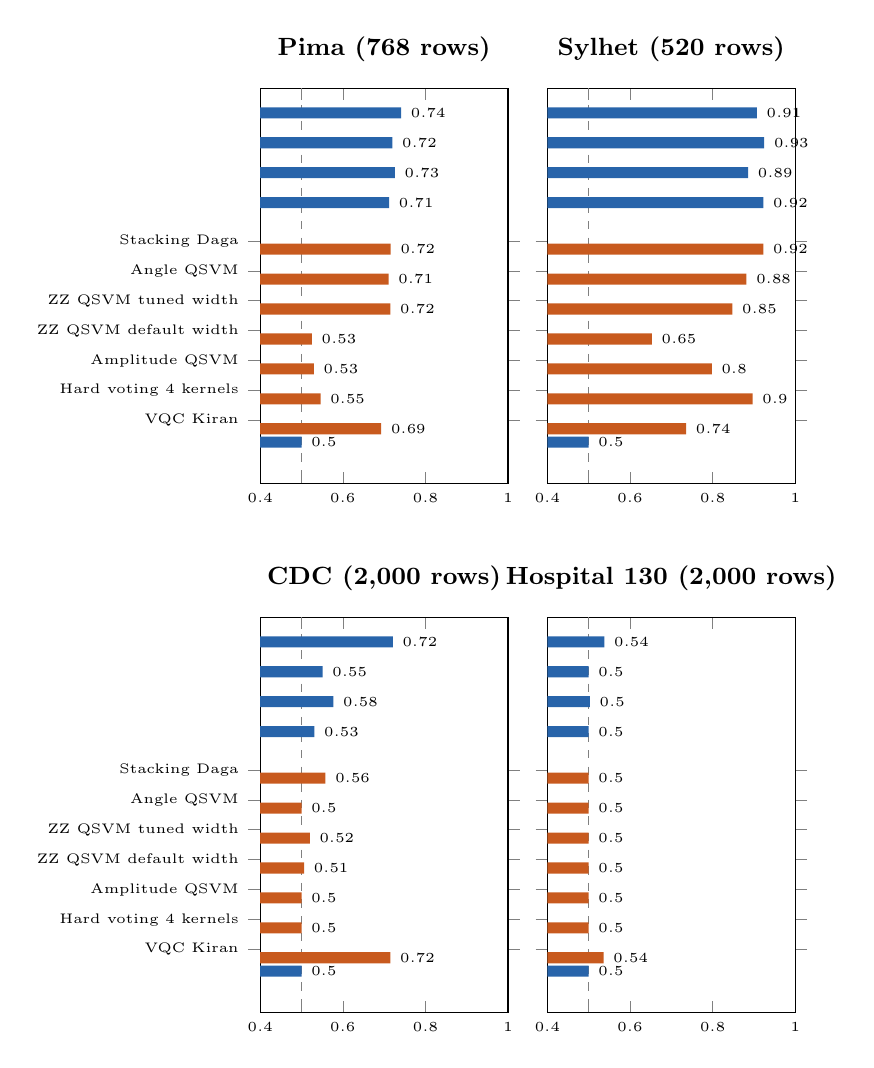
\begin{tikzpicture}\begin{groupplot}[group style={group size=2 by 2,horizontal sep=0.5cm,vertical sep=1.7cm,yticklabels at=edge left},xbar,width=0.39\linewidth,height=6.6cm,xmin=0.4,xmax=1.0,/pgf/bar width=4pt,symbolic y coords={RF tuned threshold,Random Forest,Logistic Regression,RBF-SVM ref,Stacking Daga,Angle QSVM,ZZ QSVM tuned width,ZZ QSVM default width,Amplitude QSVM,Hard voting 4 kernels,VQC Kiran,Always majority},ytick=data,y dir=reverse,yticklabel style={font=\tiny},xticklabel style={font=\tiny},title style={font=\small\bfseries},nodes near coords,nodes near coords style={font=\tiny,/pgf/number format/.cd,fixed,precision=2},point meta=x,extra x ticks={0.5},extra x tick labels={},extra x tick style={grid=major,grid style={dashed,gray}},clip=true]
\nextgroupplot[title={Pima (768 rows)}]
\addplot[fill=cq,draw=none] coordinates {(0.716,Stacking Daga) (0.711,Angle QSVM) (0.715,ZZ QSVM tuned width) (0.525,ZZ QSVM default width) (0.530,Amplitude QSVM) (0.546,Hard voting 4 kernels) (0.693,VQC Kiran)};
\addplot[fill=cc,draw=none] coordinates {(0.741,RF tuned threshold) (0.720,Random Forest) (0.726,Logistic Regression) (0.712,RBF-SVM ref) (0.500,Always majority)};
\nextgroupplot[title={Sylhet (520 rows)}]
\addplot[fill=cq,draw=none] coordinates {(0.923,Stacking Daga) (0.882,Angle QSVM) (0.848,ZZ QSVM tuned width) (0.653,ZZ QSVM default width) (0.798,Amplitude QSVM) (0.897,Hard voting 4 kernels) (0.736,VQC Kiran)};
\addplot[fill=cc,draw=none] coordinates {(0.907,RF tuned threshold) (0.925,Random Forest) (0.886,Logistic Regression) (0.923,RBF-SVM ref) (0.500,Always majority)};
\nextgroupplot[title={CDC (2,000 rows)}]
\addplot[fill=cq,draw=none] coordinates {(0.558,Stacking Daga) (0.500,Angle QSVM) (0.520,ZZ QSVM tuned width) (0.506,ZZ QSVM default width) (0.500,Amplitude QSVM) (0.500,Hard voting 4 kernels) (0.715,VQC Kiran)};
\addplot[fill=cc,draw=none] coordinates {(0.721,RF tuned threshold) (0.551,Random Forest) (0.577,Logistic Regression) (0.531,RBF-SVM ref) (0.500,Always majority)};
\nextgroupplot[title={Hospital 130 (2,000 rows)}]
\addplot[fill=cq,draw=none] coordinates {(0.500,Stacking Daga) (0.500,Angle QSVM) (0.500,ZZ QSVM tuned width) (0.500,ZZ QSVM default width) (0.500,Amplitude QSVM) (0.500,Hard voting 4 kernels) (0.536,VQC Kiran)};
\addplot[fill=cc,draw=none] coordinates {(0.538,RF tuned threshold) (0.500,Random Forest) (0.503,Logistic Regression) (0.500,RBF-SVM ref) (0.500,Always majority)};
\end{groupplot}\end{tikzpicture}

\caption{Clean balanced accuracy. \textcolor{cq}{Orange} = quantum or quantum-based; \textcolor{cc}{blue} = classical; dashed line = chance (0.5).}\end{figure}
\begin{table}[H]\centering\scriptsize\caption{Clean results, mean of 15 folds. Best non-trivial balanced accuracy in bold.}
\begin{tabular}{lccccc}
\toprule Model & Bal.\ acc & Recall & Specificity & AUC & Accuracy\\\midrule
\multicolumn{6}{l}{\textbf{Pima (768 rows)} --- `always guess the biggest group'' scores 0.651 accuracy}\\
Kotha: DiaBeats RF (threshold by inner CV) & \textbf{0.741} & 0.760 & 0.722 & 0.825 & 0.735\\
Daga: Random Forest & 0.720 & 0.586 & 0.853 & 0.824 & 0.760\\
Daga: Logistic Regression & 0.726 & 0.571 & 0.881 & 0.832 & 0.773\\
Daga: RBF-SVM & 0.712 & 0.556 & 0.869 & 0.822 & 0.760\\
Daga: OOF-Stacking (LR meta) & 0.716 & 0.567 & 0.865 & 0.830 & 0.761\\
Daga: Angle-QSVM & 0.711 & 0.552 & 0.870 & 0.832 & 0.759\\
Yadav: ZZ-QSVM (linear) bw=inner-CV & 0.715 & 0.556 & 0.874 & 0.823 & 0.763\\
Daga: ZZ-QSVM & 0.525 & 0.082 & 0.967 & 0.668 & 0.658\\
Daga: Amplitude-QSVM & 0.530 & 0.138 & 0.921 & 0.657 & 0.648\\
Daga: Hard-Voting (4 kernels) & 0.546 & 0.128 & 0.964 & 0.734 & 0.672\\
Kiran: HQCAN VQC (4q, 2 layers) & 0.693 & 0.691 & 0.695 & 0.767 & 0.694\\
Daga: Majority class & 0.500 & 0.000 & 1.000 & 0.500 & 0.651\\
\midrule\multicolumn{6}{l}{\textbf{Sylhet (520 rows)} --- `always guess the biggest group'' scores 0.615 accuracy}\\
Kotha: DiaBeats RF (threshold by inner CV) & 0.907 & 0.910 & 0.904 & 0.971 & 0.907\\
Daga: Random Forest & \textbf{0.925} & 0.943 & 0.908 & 0.972 & 0.930\\
Daga: Logistic Regression & 0.886 & 0.914 & 0.857 & 0.952 & 0.893\\
Daga: RBF-SVM & 0.923 & 0.940 & 0.905 & 0.972 & 0.928\\
Daga: OOF-Stacking (LR meta) & 0.923 & 0.929 & 0.917 & 0.969 & 0.924\\
Daga: Angle-QSVM & 0.882 & 0.918 & 0.846 & 0.958 & 0.888\\
Yadav: ZZ-QSVM (linear) bw=inner-CV & 0.848 & 0.878 & 0.817 & 0.942 & 0.856\\
Daga: ZZ-QSVM & 0.653 & 0.985 & 0.322 & 0.792 & 0.733\\
Daga: Amplitude-QSVM & 0.798 & 0.903 & 0.693 & 0.900 & 0.823\\
Daga: Hard-Voting (4 kernels) & 0.897 & 0.939 & 0.854 & 0.932 & 0.907\\
Kiran: HQCAN VQC (4q, 2 layers) & 0.736 & 0.760 & 0.712 & 0.829 & 0.740\\
Daga: Majority class & 0.500 & 1.000 & 0.000 & 0.500 & 0.619\\
\midrule\multicolumn{6}{l}{\textbf{CDC (2,000 rows)} --- `always guess the biggest group'' scores 0.860 accuracy}\\
Kotha: DiaBeats RF (threshold by inner CV) & \textbf{0.721} & 0.748 & 0.694 & 0.796 & 0.701\\
Daga: Random Forest & 0.551 & 0.120 & 0.983 & 0.801 & 0.862\\
Daga: Logistic Regression & 0.577 & 0.180 & 0.974 & 0.818 & 0.863\\
Daga: RBF-SVM & 0.531 & 0.071 & 0.990 & 0.750 & 0.862\\
Daga: OOF-Stacking (LR meta) & 0.558 & 0.133 & 0.982 & 0.756 & 0.863\\
Daga: Angle-QSVM & 0.500 & 0.000 & 1.000 & 0.717 & 0.860\\
Yadav: ZZ-QSVM (linear) bw=inner-CV & 0.520 & 0.049 & 0.992 & 0.704 & 0.860\\
Daga: ZZ-QSVM & 0.506 & 0.014 & 0.998 & 0.684 & 0.860\\
Daga: Amplitude-QSVM & 0.500 & 0.000 & 1.000 & 0.692 & 0.860\\
Daga: Hard-Voting (4 kernels) & 0.500 & 0.000 & 1.000 & 0.534 & 0.860\\
Kiran: HQCAN VQC (4q, 2 layers) & 0.715 & 0.714 & 0.716 & 0.786 & 0.716\\
Daga: Majority class & 0.500 & 0.000 & 1.000 & 0.500 & 0.860\\
\midrule\multicolumn{6}{l}{\textbf{Hospital 130 (2,000 rows)} --- `always guess the biggest group'' scores 0.912 accuracy}\\
Kotha: DiaBeats RF (threshold by inner CV) & \textbf{0.538} & 0.437 & 0.640 & 0.572 & 0.622\\
Daga: Random Forest & 0.500 & 0.000 & 0.999 & 0.583 & 0.912\\
Daga: Logistic Regression & 0.503 & 0.009 & 0.996 & 0.600 & 0.909\\
Daga: RBF-SVM & 0.500 & 0.000 & 1.000 & 0.548 & 0.912\\
Daga: OOF-Stacking (LR meta) & 0.500 & 0.000 & 1.000 & 0.512 & 0.912\\
Daga: Angle-QSVM & 0.500 & 0.000 & 1.000 & 0.497 & 0.912\\
Yadav: ZZ-QSVM (linear) bw=inner-CV & 0.500 & 0.000 & 1.000 & 0.504 & 0.912\\
Daga: ZZ-QSVM & 0.500 & 0.000 & 1.000 & 0.535 & 0.912\\
Daga: Amplitude-QSVM & 0.500 & 0.000 & 1.000 & 0.519 & 0.912\\
Daga: Hard-Voting (4 kernels) & 0.500 & 0.000 & 1.000 & 0.500 & 0.912\\
Kiran: HQCAN VQC (4q, 2 layers) & 0.536 & 0.497 & 0.576 & 0.553 & 0.569\\
Daga: Majority class & 0.500 & 0.000 & 1.000 & 0.500 & 0.912\\

\bottomrule\end{tabular}
\end{table}
\begin{figure}[H]\centering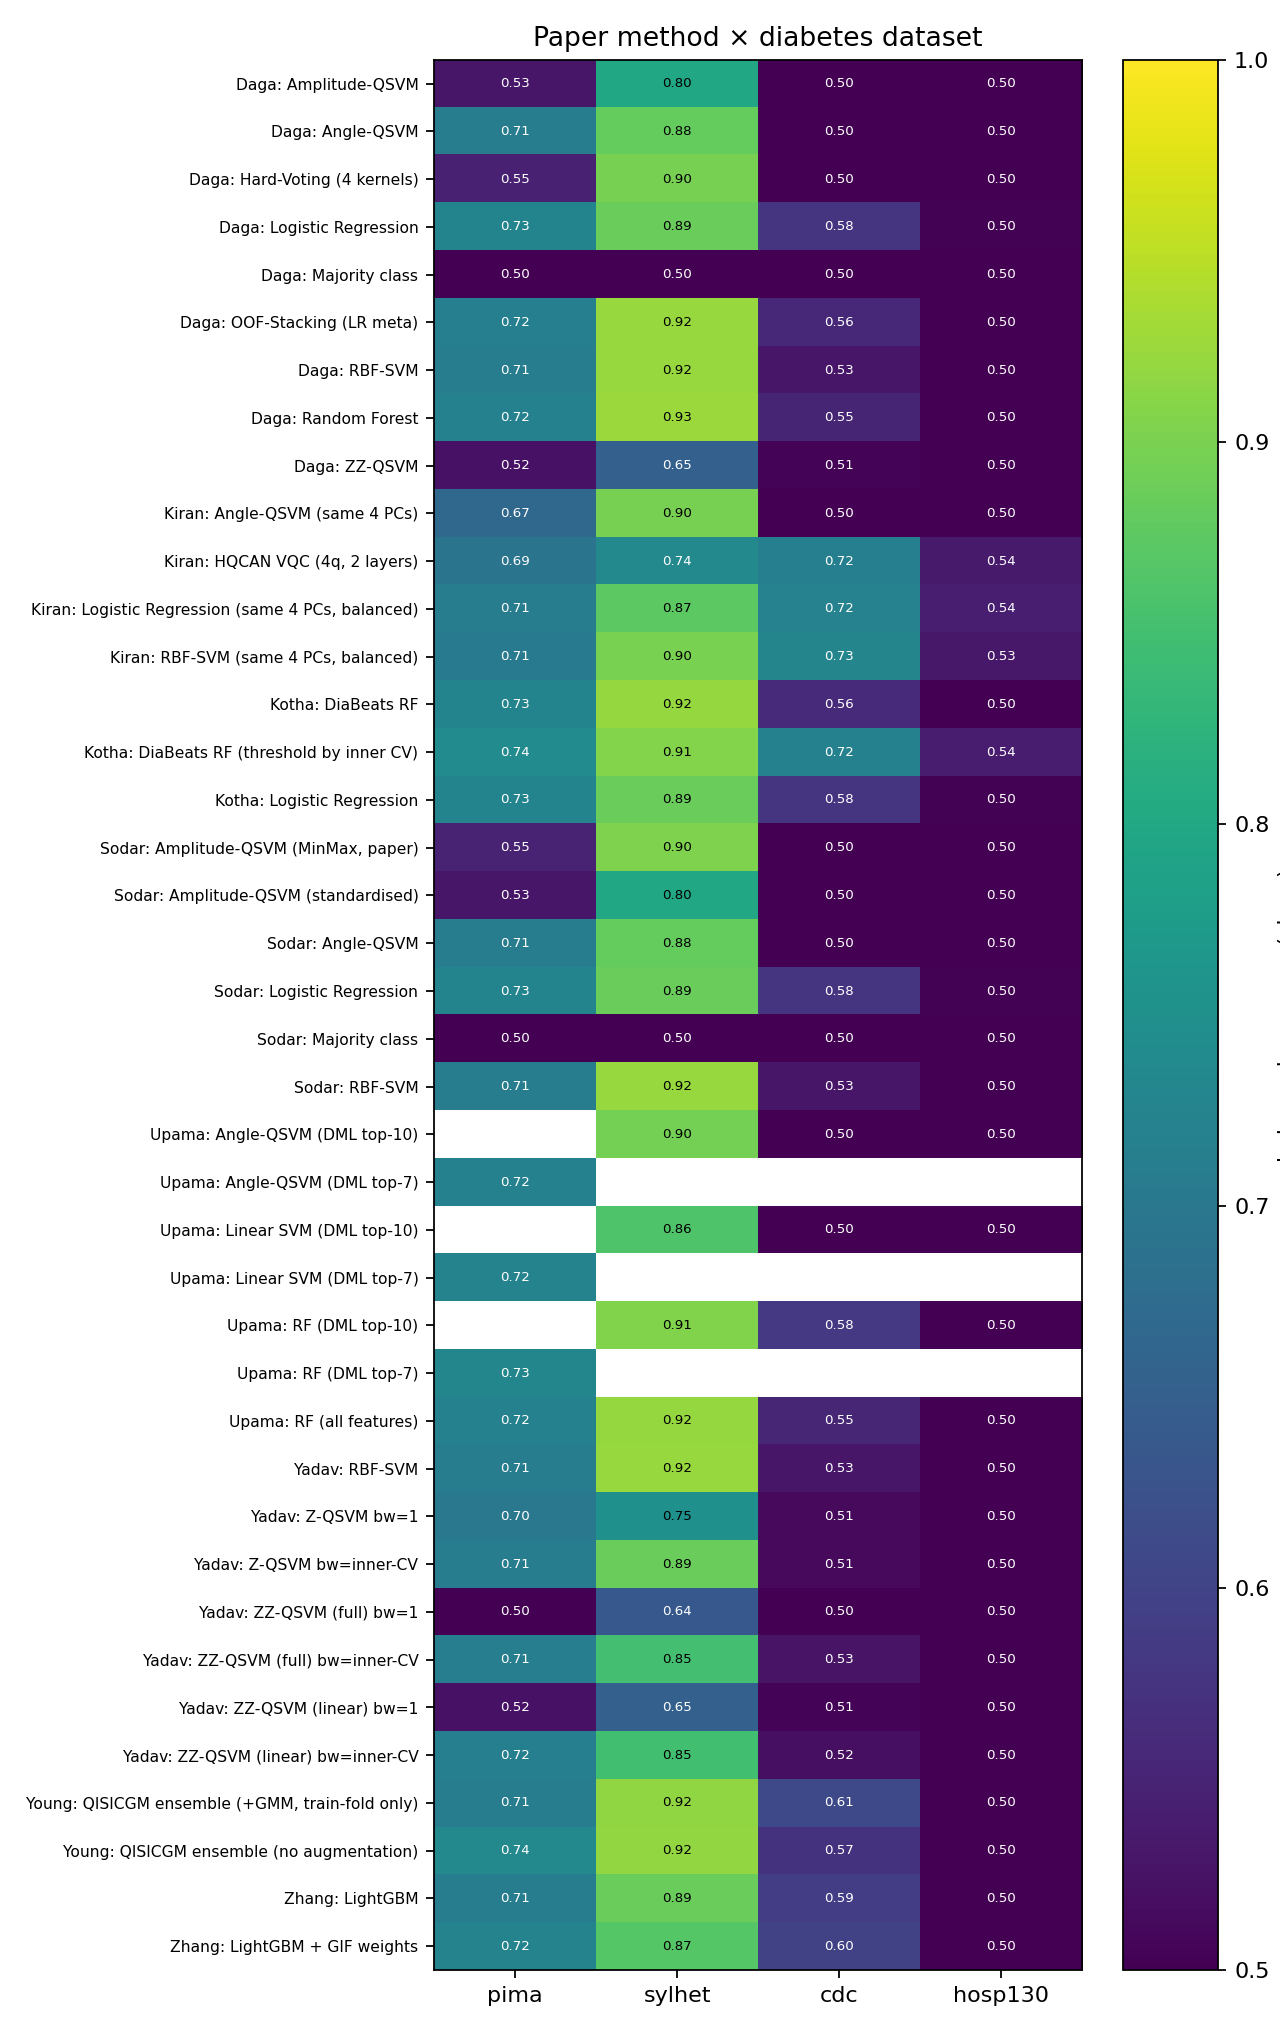
\includegraphics[width=0.9\textwidth]{09_heatmap_balanced_accuracy.png}
\caption{Notebook-generated heatmap of balanced accuracy for every method and dataset (all models, not only the selected ones).}\end{figure}

\subsection{Pima}
Classical models and the Angle quantum kernel all sit between 0.71 and 0.74; the best is Kotha's random forest with a tuned decision threshold (\mPimaKothaThrba). ZZ (\mPimaZZba), Amplitude (\mPimaAmpba) and hard voting (\mPimaHVba) are close to chance. Paper-style and clean accuracies agree closely for Daga's models (stacking gap \mDagaStackGap), so Pima has no big leak.

\subsection{Sylhet: the duplicate leak}
\begin{figure}[H]\centering
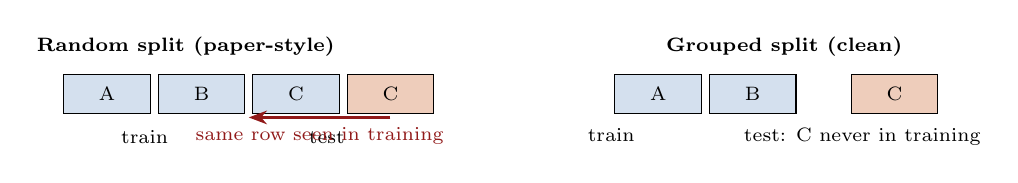
\begin{tikzpicture}[font=\scriptsize,r/.style={draw,minimum width=1.1cm,minimum height=0.5cm}]
\node at (-3.2,1.6){\textbf{Random split (paper-style)}};
\foreach \i/\t in {0/A,1/B,2/C}{\node[r,fill=cc!20] at (-4.2+1.2*\i,1){\t};}
\node[r,fill=cq!30] at (-0.6,1){C};
\node at (-2.6,0.45){train \hspace{1.6cm} test};
\draw[-{Stealth},thick,bad] (-0.6,0.7)--(-2.4,0.7) node[midway,below]{same row seen in training};
\node at (4.4,1.6){\textbf{Grouped split (clean)}};
\foreach \i/\t in {0/A,1/B}{\node[r,fill=cc!20] at (2.8+1.2*\i,1){\t};}
\node[r,fill=cq!30] at (5.8,1){C};\node at (4.4,0.45){train \hspace{1.2cm} test: C never in training};
\end{tikzpicture}\caption{Why duplicates inflate scores: a model that learns rows by heart can score well on a test row it has already seen.}\end{figure}
Clean balanced accuracy: random forest \mSylRFba, RBF-SVM \mSylRBFba, stacking \mSylStackba, Angle QSVM \mSylAngleba. ZZ with default width reaches \mSylZZba because it answers ``diabetic'' almost always (recall \mSylZZrec, specificity \mSylZZspec).
\begin{figure}[H]\centering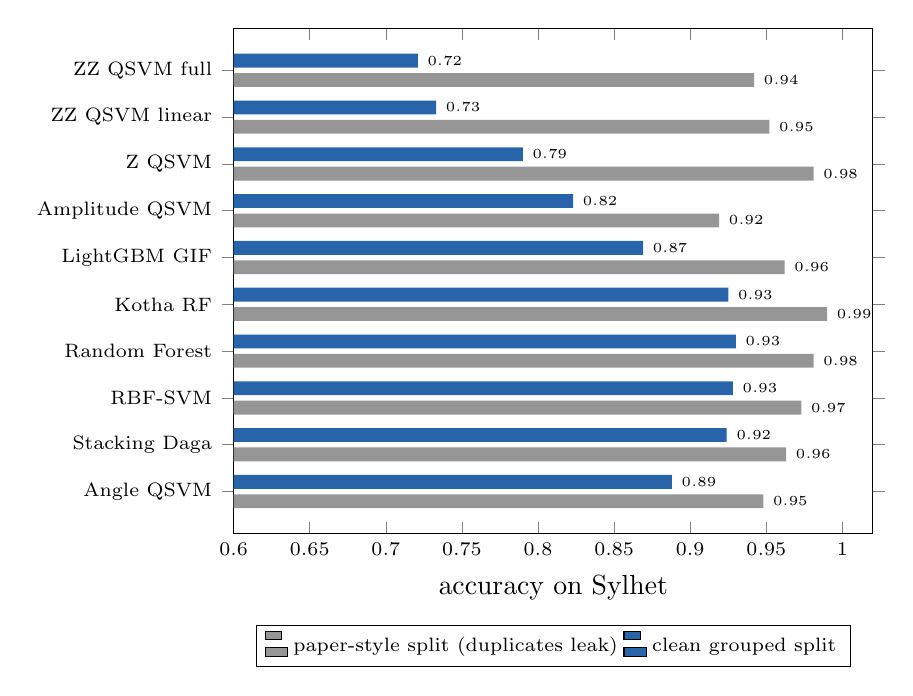
\begin{tikzpicture}\begin{axis}[xbar,width=0.8\linewidth,height=8cm,xmin=0.6,xmax=1.02,/pgf/bar width=5pt,symbolic y coords={ZZ QSVM full,ZZ QSVM linear,Z QSVM,Amplitude QSVM,LightGBM GIF,Kotha RF,Random Forest,RBF-SVM,Stacking Daga,Angle QSVM},ytick=data,y dir=reverse,yticklabel style={font=\scriptsize},xticklabel style={font=\scriptsize},xlabel={accuracy on Sylhet},legend style={at={(0.5,-0.18)},anchor=north,legend columns=2,font=\scriptsize},nodes near coords,nodes near coords style={font=\tiny,/pgf/number format/.cd,fixed,precision=2},point meta=x]
\addplot[fill=cp,draw=none] coordinates {(0.942,ZZ QSVM full) (0.952,ZZ QSVM linear) (0.981,Z QSVM) (0.919,Amplitude QSVM) (0.962,LightGBM GIF) (0.990,Kotha RF) (0.981,Random Forest) (0.973,RBF-SVM) (0.963,Stacking Daga) (0.948,Angle QSVM)};
\addplot[fill=cc,draw=none] coordinates {(0.721,ZZ QSVM full) (0.733,ZZ QSVM linear) (0.790,Z QSVM) (0.823,Amplitude QSVM) (0.869,LightGBM GIF) (0.925,Kotha RF) (0.930,Random Forest) (0.928,RBF-SVM) (0.924,Stacking Daga) (0.888,Angle QSVM)};
\legend{paper-style split (duplicates leak),clean grouped split}
\end{axis}\end{tikzpicture}
\caption{Accuracy on Sylhet, paper-style (grey) vs clean (blue).}\end{figure}
\begin{table}[H]\centering\small\caption{Sylhet leak size (accuracy points, paper-style minus clean). Gaps use unrounded values, so they can differ by 0.1 from the rounded columns.}
\begin{tabular}{lccc}
\toprule Model & Paper-style & Clean & Gap (points)\\\midrule
Yadav: ZZ-QSVM (full) bw=1 & 0.942 & 0.721 & +22.2 \\
Yadav: ZZ-QSVM (linear) bw=1 & 0.952 & 0.733 & +21.9 \\
Yadav: Z-QSVM bw=1 & 0.981 & 0.790 & +19.0 \\
Daga: Amplitude-QSVM & 0.919 & 0.823 & +9.6 \\
Zhang: LightGBM + GIF weights & 0.962 & 0.869 & +9.3 \\
Kotha: DiaBeats RF & 0.990 & 0.925 & +6.6 \\
Daga: Random Forest & 0.981 & 0.930 & +5.1 \\
Daga: RBF-SVM & 0.973 & 0.928 & +4.5 \\
Daga: OOF-Stacking (LR meta) & 0.963 & 0.924 & +4.0 \\
Daga: Angle-QSVM & 0.948 & 0.888 & +6.0 \\

\bottomrule\end{tabular}
\end{table}
Models that can learn rows by heart (ZZ kernels at width 1) gain most. Part of the gap also comes from comparing a single split with 5-fold CV; for Daga's pooled-CV models the gap is purely the grouping effect.

\subsection{CDC and Hospital 130: models that never say ``sick''}
\begin{figure}[H]\centering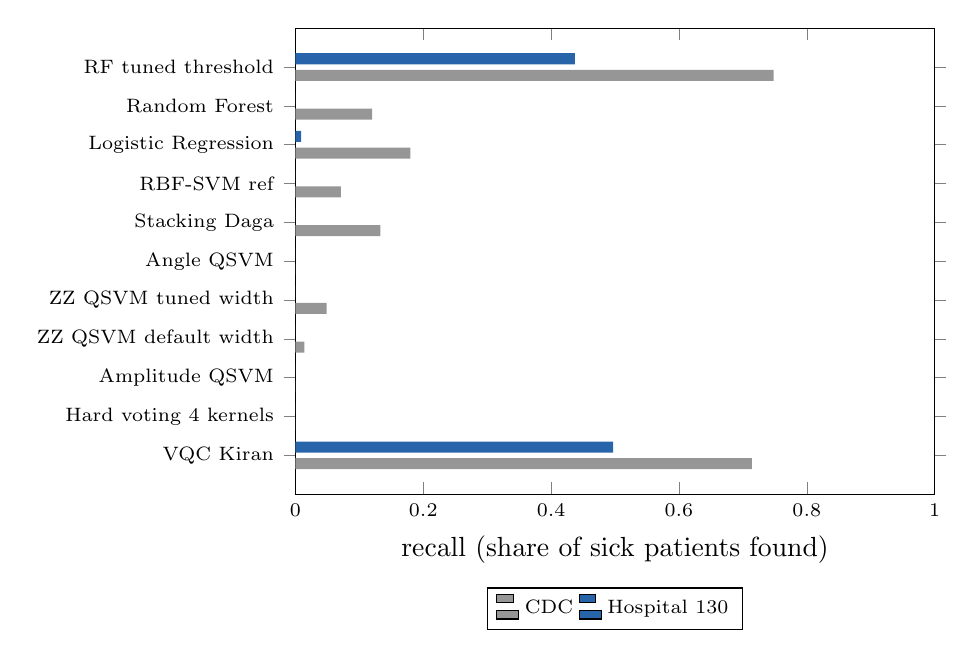
\begin{tikzpicture}\begin{axis}[xbar,width=0.8\linewidth,height=7.5cm,xmin=0,xmax=1,/pgf/bar width=4pt,symbolic y coords={RF tuned threshold,Random Forest,Logistic Regression,RBF-SVM ref,Stacking Daga,Angle QSVM,ZZ QSVM tuned width,ZZ QSVM default width,Amplitude QSVM,Hard voting 4 kernels,VQC Kiran},ytick=data,y dir=reverse,yticklabel style={font=\scriptsize},xticklabel style={font=\scriptsize},xlabel={recall (share of sick patients found)},legend style={at={(0.5,-0.2)},anchor=north,legend columns=2,font=\scriptsize}]
\addplot[fill=cp,draw=none] coordinates {(0.748,RF tuned threshold) (0.120,Random Forest) (0.180,Logistic Regression) (0.071,RBF-SVM ref) (0.133,Stacking Daga) (0.000,Angle QSVM) (0.049,ZZ QSVM tuned width) (0.014,ZZ QSVM default width) (0.000,Amplitude QSVM) (0.000,Hard voting 4 kernels) (0.714,VQC Kiran)};
\addplot[fill=cc,draw=none] coordinates {(0.437,RF tuned threshold) (0.000,Random Forest) (0.009,Logistic Regression) (0.000,RBF-SVM ref) (0.000,Stacking Daga) (0.000,Angle QSVM) (0.000,ZZ QSVM tuned width) (0.000,ZZ QSVM default width) (0.000,Amplitude QSVM) (0.000,Hard voting 4 kernels) (0.497,VQC Kiran)};
\legend{CDC,Hospital 130}
\end{axis}\end{tikzpicture}
\caption{Recall (sick people found). Many bars are zero: those models just guess the biggest group.}\end{figure}
On CDC only class-weighted or threshold-tuned models work (Kiran's balanced RBF-SVM: balanced accuracy \mCdcKiranRBFba, recall \mCdcKiranRBFrec). Plain RBF-SVM scores \mCdcRBFba. Hospital 130 stays near chance for everyone (best \mHospBestba).

\subsection{Statistical tests against RBF-SVM}
\begin{table}[H]\centering\scriptsize\caption{Paired tests on balanced accuracy (Nadeau--Bengio, Holm-adjusted per dataset). ``Better'' on CDC means better than a plain RBF-SVM that finds almost no positives; the cause is class weighting, not the quantum or classical type.}
\begin{tabular}{lcccl}
\toprule Model & Mean diff & Raw $p$ & Holm $p$ & Verdict\\\midrule
\multicolumn{5}{l}{\textbf{Pima (768 rows)}}\\
Daga: OOF-Stacking (LR meta) & +0.004 & 0.598 & 1.000 & no clear difference\\
Daga: Angle-QSVM & -0.001 & 0.912 & 1.000 & no clear difference\\
Daga: ZZ-QSVM & -0.188 & 0.000 & $<$0.0001 & \BAD{worse}\\
Daga: Amplitude-QSVM & -0.183 & 0.000 & $<$0.0001 & \BAD{worse}\\
Daga: Hard-Voting (4 kernels) & -0.166 & 0.000 & $<$0.0001 & \BAD{worse}\\
Yadav: ZZ-QSVM (linear) bw=inner-CV & +0.003 & 0.868 & 1.000 & no clear difference\\
Yadav: ZZ-QSVM (linear) bw=1 & -0.188 & 0.000 & $<$0.0001 & \BAD{worse}\\
Kiran: HQCAN VQC (4q, 2 layers) & -0.019 & 0.270 & 1.000 & no clear difference\\
Kiran: RBF-SVM (same 4 PCs, balanced) & -0.005 & 0.837 & 1.000 & no clear difference\\
Kotha: DiaBeats RF (threshold by inner CV) & +0.029 & 0.256 & 1.000 & no clear difference\\
\midrule\multicolumn{5}{l}{\textbf{Sylhet (520 rows)}}\\
Daga: OOF-Stacking (LR meta) & +0.000 & 0.993 & 1.000 & no clear difference\\
Daga: Angle-QSVM & -0.041 & 0.109 & 1.000 & no clear difference\\
Daga: ZZ-QSVM & -0.270 & 0.000 & 0.001 & \BAD{worse}\\
Daga: Amplitude-QSVM & -0.125 & 0.010 & 0.290 & no clear difference\\
Daga: Hard-Voting (4 kernels) & -0.026 & 0.198 & 1.000 & no clear difference\\
Yadav: ZZ-QSVM (linear) bw=inner-CV & -0.075 & 0.058 & 1.000 & no clear difference\\
Yadav: ZZ-QSVM (linear) bw=1 & -0.270 & 0.000 & 0.001 & \BAD{worse}\\
Kiran: HQCAN VQC (4q, 2 layers) & -0.187 & 0.022 & 0.603 & no clear difference\\
Kiran: RBF-SVM (same 4 PCs, balanced) & -0.023 & 0.198 & 1.000 & no clear difference\\
Kotha: DiaBeats RF (threshold by inner CV) & -0.016 & 0.601 & 1.000 & no clear difference\\
\midrule\multicolumn{5}{l}{\textbf{CDC (2,000 rows)}}\\
Daga: OOF-Stacking (LR meta) & +0.027 & 0.003 & 0.077 & no clear difference\\
Daga: Angle-QSVM & -0.031 & 0.010 & 0.231 & no clear difference\\
Daga: ZZ-QSVM & -0.025 & 0.052 & 0.516 & no clear difference\\
Daga: Amplitude-QSVM & -0.031 & 0.010 & 0.231 & no clear difference\\
Daga: Hard-Voting (4 kernels) & -0.031 & 0.010 & 0.231 & no clear difference\\
Yadav: ZZ-QSVM (linear) bw=inner-CV & -0.010 & 0.383 & 1.000 & no clear difference\\
Yadav: ZZ-QSVM (linear) bw=1 & -0.025 & 0.052 & 0.516 & no clear difference\\
Kiran: HQCAN VQC (4q, 2 layers) & +0.184 & 0.000 & $<$0.0001 & \OK{better}\\
Kiran: RBF-SVM (same 4 PCs, balanced) & +0.197 & 0.000 & $<$0.0001 & \OK{better}\\
Kotha: DiaBeats RF (threshold by inner CV) & +0.190 & 0.000 & $<$0.0001 & \OK{better}\\
\midrule\multicolumn{5}{l}{\textbf{Hospital 130 (2,000 rows)}}\\
Daga: OOF-Stacking (LR meta) & +0.000 & 1.000 & 1.000 & no clear difference\\
Daga: Angle-QSVM & +0.000 & 1.000 & 1.000 & no clear difference\\
Daga: ZZ-QSVM & +0.000 & 1.000 & 1.000 & no clear difference\\
Daga: Amplitude-QSVM & +0.000 & 1.000 & 1.000 & no clear difference\\
Daga: Hard-Voting (4 kernels) & +0.000 & 1.000 & 1.000 & no clear difference\\
Yadav: ZZ-QSVM (linear) bw=inner-CV & +0.000 & 1.000 & 1.000 & no clear difference\\
Yadav: ZZ-QSVM (linear) bw=1 & +0.000 & 1.000 & 1.000 & no clear difference\\
Kiran: HQCAN VQC (4q, 2 layers) & +0.036 & 0.180 & 1.000 & no clear difference\\
Kiran: RBF-SVM (same 4 PCs, balanced) & +0.032 & 0.085 & 1.000 & no clear difference\\
Kotha: DiaBeats RF (threshold by inner CV) & +0.038 & 0.059 & 1.000 & no clear difference\\

\bottomrule\end{tabular}
\end{table}
Counts over all models tested: Pima \npimaworse{} worse / \npimaNS{} no difference; Sylhet \nsylhetworse{} worse / \nsylhetNS{} no difference; CDC \ncdcbetter{} better / \ncdcNS{} no difference; Hospital 130 \nhospNS{} no difference. \textbf{No model beats RBF-SVM on Pima, Sylhet or Hospital 130.} The ``worse'' cases are mostly ZZ/Amplitude with default settings, plus the majority-class guess.

\subsection{Zhang: label noise}
\begin{figure}[H]\centering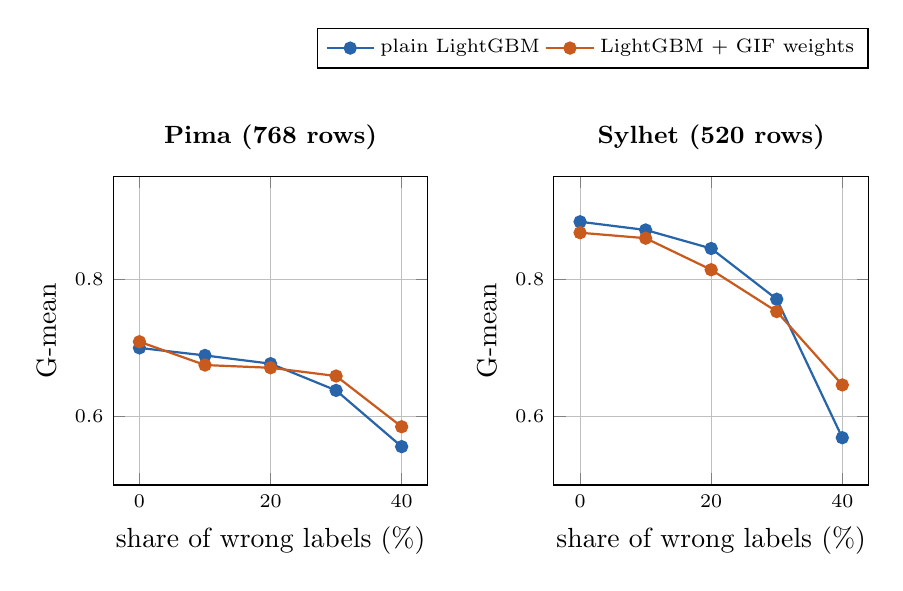
\begin{tikzpicture}\begin{groupplot}[group style={group size=2 by 1,horizontal sep=1.6cm},width=0.46\linewidth,height=5.5cm,xlabel={share of wrong labels (\%)},ylabel={G-mean},ymin=0.5,ymax=0.95,grid=major,tick label style={font=\scriptsize},title style={font=\small\bfseries},legend style={font=\scriptsize,at={(1,1.35)},anchor=south east,legend columns=2}]
\nextgroupplot[title={Pima (768 rows)}]
\addplot[color=cc,mark=*,thick] coordinates {(0,0.700) (10,0.689) (20,0.677) (30,0.638) (40,0.556)};
\addplot[color=cq,mark=*,thick] coordinates {(0,0.709) (10,0.675) (20,0.671) (30,0.659) (40,0.585)};
\nextgroupplot[title={Sylhet (520 rows)}]
\addplot[color=cc,mark=*,thick] coordinates {(0,0.884) (10,0.872) (20,0.845) (30,0.771) (40,0.569)};
\addplot[color=cq,mark=*,thick] coordinates {(0,0.868) (10,0.860) (20,0.814) (30,0.753) (40,0.646)};
\legend{plain LightGBM,LightGBM + GIF weights}
\end{groupplot}\end{tikzpicture}
\caption{G-mean as labels are corrupted. Single curves, no significance test.}\end{figure}
At 40\% noise GIF weights give G-mean \zhpimaLightGBMGIFweights{} vs \zhpimaLightGBM{} (Pima) and \zhsylhetLightGBMGIFweights{} vs \zhsylhetLightGBM{} (Sylhet). On Sylhet GIF is worse at low noise, so the effect is mixed. Zhang's paper reports about 0.6 on private audio data, not comparable.

\subsection{Zhang: paper-style test on all four datasets}
Here we copy Zhang's own set-up (one split, labels flipped on purpose) and look at both balanced accuracy and recall. Numbers are averages over the folds, taken from \texttt{04\_zhang.csv}.
\begin{table}[H]\centering\small\caption{Zhang, paper-style test. Plain LightGBM vs LightGBM with GIF weights, when 0\%, 20\% or 40\% of the training labels are wrong.}
\begin{tabular}{llcccccc}
\toprule & & \multicolumn{3}{c}{Balanced accuracy} & \multicolumn{3}{c}{Recall}\\
Dataset & Model & 0\% noise & 20\% & 40\% & 0\% & 20\% & 40\%\\\midrule
Pima & plain & 0.712 & 0.678 & 0.545 & 0.582 & 0.574 & 0.495\\
Pima & + GIF & 0.732 & 0.712 & 0.638 & 0.612 & 0.600 & 0.574\\
\midrule
Sylhet & plain & 0.972 & 0.896 & 0.653 & 0.969 & 0.913 & 0.681\\
Sylhet & + GIF & 0.964 & 0.891 & 0.735 & 0.953 & 0.881 & 0.716\\
\midrule
CDC & plain & 0.583 & 0.587 & 0.547 & 0.201 & 0.229 & 0.315\\
CDC & + GIF & 0.591 & 0.565 & 0.577 & 0.222 & 0.179 & 0.304\\
\midrule
Hospital 130 & plain & 0.502 & 0.500 & 0.505 & 0.006 & 0.011 & 0.211\\
Hospital 130 & + GIF & 0.500 & 0.508 & 0.536 & 0.011 & 0.051 & 0.250\\
\bottomrule\end{tabular}

\end{table}
\begin{itemize}[leftmargin=1.5em]
\item GIF weights help on Pima at every noise level (balanced accuracy 0.732 vs 0.712 with clean labels, 0.638 vs 0.545 at 40\% noise).
\item On Sylhet GIF is a little worse with clean labels and a little better at 40\% noise. The effect is mixed.
\item On CDC and Hospital 130 both models are close to chance (balanced accuracy 0.50 to 0.59) and find very few sick people. GIF weights do not fix that.
\item These are single runs on one split. We did not test the differences, so treat them as hints only.
\end{itemize}

\subsection{Young: made-up test rows make the score look better}
Young's method adds computer-made (synthetic) patients, and the paper's test set also contains some of them. Those rows are easy to get right. We scored the same model twice: once on the paper-style test set and once on real people only.
\begin{table}[H]\centering\small\caption{Young's QISICGM ensemble. Left: paper-style test set that includes made-up rows. Right: real rows only. Mean over 5 folds (seed 42), from \texttt{02\_young.csv}.}
\begin{tabular}{lcccccc}
\toprule & \multicolumn{3}{c}{Paper-style test (with made-up rows)} & \multicolumn{3}{c}{Real rows only}\\
Dataset & Accuracy & Bal.\ acc. & Recall & Accuracy & Bal.\ acc. & Recall\\\midrule
Pima & 0.897 & 0.767 & 0.971 & 0.675 & 0.725 & 0.885\\
Sylhet & 0.996 & 0.987 & 0.998 & 0.985 & 0.983 & 0.992\\
CDC & 0.957 & 0.951 & 0.963 & 0.851 & 0.622 & 0.304\\
Hospital 130 & 0.972 & 0.977 & 0.967 & 0.902 & 0.506 & 0.026\\
\bottomrule\end{tabular}
\end{table}
\begin{itemize}[leftmargin=1.5em]
\item \BAD{CDC:} balanced accuracy drops from 0.951 to 0.622 and recall from 0.963 to 0.304 once the made-up rows are removed.
\item \BAD{Hospital 130:} balanced accuracy drops from 0.977 to 0.506 (chance) and recall from 0.967 to 0.026. The model finds almost no real patients who return.
\item Pima: balanced accuracy goes from 0.767 to 0.725, and accuracy from 0.897 to 0.675.
\item Sylhet: almost no change (0.987 to 0.983), but Sylhet also has the duplicate-row problem described above.
\end{itemize}
So the very high paper-style numbers mainly show how easy the made-up rows are.

\section{Comparison with the original papers}
\begin{table}[H]\centering\scriptsize\caption{Paper-style results (bootstrap 95\% range of accuracy) vs claimed accuracy. Claims from \texttt{recheck/results/paper\_claims\_v2.csv}. N = test rows; ranges for small holdouts are wide.}
\begin{tabular}{llrcccl}
\toprule Paper & Setting & N & Claimed & Ours [95\%] & Diff & Verdict\\\midrule
Daga & Pima, stacking accuracy & 768 & 0.766 & 0.759 [0.731, 0.789] & -0.007 & \OK{claim inside our 95\% range}\\
Daga & Pima, Angle QSVM accuracy & 768 & 0.763 & 0.758 [0.728, 0.789] & -0.005 & \OK{claim inside our 95\% range}\\
Daga & Pima, ZZ QSVM accuracy & 768 & 0.759 & 0.663 [0.630, 0.697] & -0.096 & \BAD{claim too high to reproduce}\\
Daga & Pima, Amplitude QSVM accuracy & 768 & 0.763 & 0.638 [0.603, 0.671] & -0.125 & \BAD{claim too high to reproduce}\\
Daga & Pima, RBF-SVM accuracy & 768 & 0.758 & 0.760 [0.731, 0.790] & +0.002 & \OK{claim inside our 95\% range}\\
Upama & Pima, SVM accuracy & 154 & 0.720 & 0.721 [0.656, 0.792] & +0.001 & \OK{claim inside our 95\% range}\\
Upama & Pima, QSVM (our Angle) & 154 & 0.650 & 0.753 [0.682, 0.818] & +0.103 & \WARN{we score higher than claim}\\
Upama & Pima, QSVM (our ZZ, width 1) & 154 & 0.650 & 0.649 [0.571, 0.727] & -0.001 & \OK{claim inside our 95\% range}\\
Upama & Pima, RF accuracy & 154 & 0.760 & 0.779 [0.714, 0.838] & +0.019 & \OK{claim inside our 95\% range}\\
Upama & Sylhet, SVM accuracy & 104 & 0.923 & 0.942 [0.894, 0.981] & +0.019 & \OK{claim inside our 95\% range}\\
Upama & Sylhet, RF accuracy & 104 & 0.971 & 0.981 [0.952, 1.000] & +0.010 & \OK{claim inside our 95\% range}\\
Upama & Sylhet, QSVM (our Angle) & 104 & 0.971 & 0.942 [0.894, 0.981] & -0.029 & \OK{claim inside our 95\% range}\\
Upama & Sylhet, QSVM (our ZZ, width 1) & 104 & 0.971 & 0.942 [0.894, 0.981] & -0.029 & \OK{claim inside our 95\% range}\\
Kotha & Pima, RF accuracy & 154 & 0.833 & 0.760 [0.695, 0.825] & -0.074 & \BAD{claim too high to reproduce}\\
Kiran & Pima, VQC accuracy & 154 & 0.997 & 0.675 [0.604, 0.747] & -0.322 & \BAD{claim too high to reproduce}\\

\bottomrule\end{tabular}
\end{table}
\begin{itemize}[leftmargin=1.5em]
\item \textbf{Daga:} stacking, Angle and RBF reproduce. ZZ and Amplitude do \emph{not} (here default scaling; the paper may have tuned them). Claimed AUC 0.734 is below every model we ran (stacking: \mDagaStackAUC), and claimed recall 0.621 is above ours (\mDagaStackRec): unexplained.
\item \textbf{Upama:} Pima results match; Sylhet scores are leak-inflated. Their QSVM$=0.65$ on Pima equals the majority rate, as our ZZ width-1 model shows.
\item \textbf{Kotha:} 0.833 not reproduced; AUC 1.00 is mathematically impossible with 25 errors in 150 (AUC $\le 0.97$).
\item \textbf{Kiran:} 99.7\% contradicts its own 4\% error rate; honest VQC gets \mKiranVQCpaperAcc--\mKiranVQCcleanAcc.
\item \textbf{Young:} claimed F1 0.8933/AUC 0.8699 rely on synthetic rows in validation folds ((268+2000)/2768 = 81.9\% ``positive''). With GMM fitted on training folds only: AUC \mYoungGMMauc, recall \mYoungGMMrec{} but specificity only \mYoungGMMspec.
\item \textbf{Zhang, Sodar, Yadav:} original data (audio, URLs, breast cancer) are out of scope; we only adapted the methods. Yadav's ``$>90\%$ on Pima'' is not supported.
\end{itemize}

\section{Comparison with earlier project phases}
\begin{figure}[H]\centering
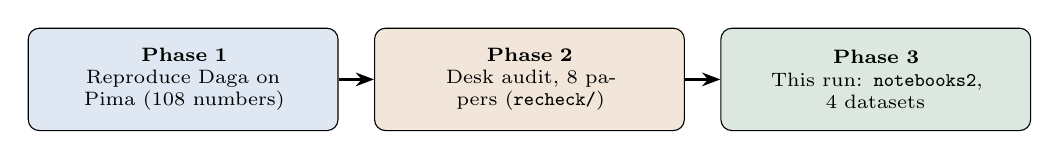
\begin{tikzpicture}[font=\scriptsize,node distance=0.45cm,b/.style={draw,rounded corners,align=center,text width=3.7cm,minimum height=1.3cm}]
\node[b,fill=cc!15](a){\textbf{Phase 1}\\Reproduce Daga on Pima (108 numbers)};
\node[b,fill=warn!15,right=of a](b2){\textbf{Phase 2}\\Desk audit, 8 papers (\texttt{recheck/})};
\node[b,fill=ok!15,right=of b2](c){\textbf{Phase 3}\\This run: \texttt{notebooks2}, 4 datasets};
\draw[-{Stealth},thick](a)--(b2);\draw[-{Stealth},thick](b2)--(c);
\end{tikzpicture}\caption{Project phases.}\end{figure}
\begin{table}[H]\centering\scriptsize\caption{Earlier results (from \texttt{recheck/DISCREPANCY\_LOG.csv}) vs this run.}
\begin{tabular}{p{2.2cm}p{4.6cm}p{6.4cm}}\toprule Topic & Earlier phase & This run\\\midrule
Upama, Sylhet RF & 98.08\% random split; 85.77\% grouped CV & paper-style \mUpamaSylRFpaper; clean \mUpamaSylRFclean. \WARN{Clean is 7 points higher than earlier 85.77\%; not yet explained (different fold design or features?).}\\
Kotha, Pima & honest CV 76.65\% acc, AUC 0.824 & \mKothaPimaCleanAcc{} acc, AUC \mKothaPimaAUC. \OK{Consistent.}\\
Kiran, Pima VQC & 64.97\% & \mKiranVQCcleanAcc{} (clean), \mKiranVQCpaperAcc{} (paper-style). Slightly higher; same conclusion.\\
Young, Pima & GMM harms precision on real patients (50.11\%) & balanced accuracy \mYoungGMMba, accuracy \mYoungGMMacc{} (floor \mPimaFloor): \OK{consistent}, many false alarms.\\
Yadav, Pima & ZZ 69.13\% vs Z 74.73\% & ZZ \mYadavZZpimaAcc{} vs Z \mYadavZpimaAcc: \OK{same direction}.\\
Sodar, Pima & raw Amplitude recall 0.0\% & recall \mSodarAmpMinMaxRec{} (MinMax), \mSodarAmpStdRec{} (standardised). \WARN{Differs; settings may differ.}\\
Daga, Pima & global Gram matrix inflates ~0.4\% & paper-style minus clean stacking accuracy: \mDagaStackGap. \WARN{No inflation visible here.}\\\bottomrule\end{tabular}\end{table}

\section{Corrections to the previous draft}
\begin{table}[H]\centering\scriptsize\begin{tabular}{p{0.3cm}p{6.2cm}p{7.5cm}}\toprule \# & Problem in the earlier draft & Correction\\\midrule
1 & ``Original claim'' column listed 98.08\% (Upama) and F1 0.940/AUC 0.932 (Young). & These were \emph{our earlier reproductions}. The papers claim 97.12\% (RF) and F1 0.8933/AUC 0.8699.\\
2 & ``ZZ-QSVM systematically underperforms''. & Only with default width 1; with tuned width ZZ ties RBF on Pima and Sylhet.\\
3 & CDC ``cost-weighted superior''. & The reference RBF finds only \mCdcRBFrec{} of positives; the gain is from class weighting.\\
4 & ``All pure QSVMs: bal.\ acc 0.500, recall 0'' on CDC. & True for Angle and Amplitude; ZZ is slightly above (e.g.\ Daga ZZ 0.506).\\
5 & ``376 rows in duplicate clusters''. & Not verified; the audit confirms only 251 unique, 269 redundant rows.\\
6 & Sylhet ``clean 90.5--92.0\%'' mixed accuracy and balanced accuracy. & Now stated separately.\\
7 & No comparison with the papers' own claims; no Hospital 130 tests; Zhang noise omitted. & Added.\\
8 & Table row groups miscounted (\texttt{multirow}). & Table rebuilt.\\
9 & Sodar ``rank-1 Gram, 85.3\%'' stated as current result. & From the earlier audit; not re-measured here.\\\bottomrule\end{tabular}\end{table}

\section{Limits and open questions}
\begin{itemize}[leftmargin=1.5em]
\item Quantum models are simulated with at most 8 qubits; CDC and Hospital 130 use 2,000-row subsamples (less power).
\item The 15 folds are correlated; corrected tests are cautious but not perfect. Paper-style holdouts of 104--154 rows give ranges of about $\pm$6 points.
\item We read only the parts of the notebook code tied to the open questions (01, 06, 08 and the authors' script), not every line, and we did not view the PDF pages by eye. The Zhang and Young tables above are single runs without significance tests.
item Not yet tested: the explanations above for Daga (IQP map, PCA scaling, hard-vote stacking) and for Upama's Sylhet gap. They need a machine with Python.
item Next steps: add an IQP kernel and a hard-vote stacker to the notebooks and rerun; add a Sylhet run on the 251 distinct rows.
\end{itemize}

\section{Conclusion}
For diabetes tabular data, tuned classical models (random forest, logistic regression, RBF-SVM) are as good as any quantum kernel we tested. Quantum kernels need tuning to avoid collapse, never gave a significant gain, and several high published numbers come from duplicate leaks, synthetic rows in validation, or are not reproducible. Report balanced accuracy and recall, use grouped splits for survey data, and compare against tuned classical baselines.

\appendix\section{How the numbers were produced}
\texttt{notebooks2/results/summary.md} (from the Colab run) was parsed by \texttt{latex\_report/gen\_part1.ps1} and \texttt{gen\_part2.ps1}, which write the files in \texttt{gen\_v2/} (tables, chart data, macros). Re-run them to refresh the report. Claimed values are from \texttt{recheck/results/paper\_claims\_v2.csv}.
\end{document}

